\paragraph{Historical agent trajectories.}
We reanalyzed 3,336 public $\tau^2$-bench runs from three systems
(GPT-4.1, o4-mini, and Claude-3.7) on 50 airline, 114 retail, and 114
telecom tasks, with four trials per task and system. Within each domain,
the compared runs share the same harness commit, tasks, and user
simulator. We also analyzed 600 SWE-agent trajectories, one per system
on each of 300 SWE-bench Lite tasks. The hierarchy is verified success,
historical recorded agent cost, then tool-call count; both failures tie.
No policy-compliance label is fabricated where the source does not
provide one. Recorded simulation duration includes simulator and service
delays and is not used as clean agent latency.

The primary $\tau^2$ statistic excludes same-seed diagonal comparisons,
leaving 12 cross-seed comparisons per task. A theory audit motivated this
amendment before the hierarchical numerical results were inspected.
Same-seed and all-16-pair statistics are sensitivity analyses. We report
pointwise percentile intervals from 10,000 complete-task bootstrap
resamples. Because these are historical benchmark tasks with only four
shared seed values per domain, the intervals are descriptive under
task-resampling assumptions, conditional on the recorded seed suite;
they do not account for arbitrary cross-task seed effects or establish
uncertainty over newly generated seeds. SWE repository dependence poses
an additional limitation. There is no multiplicity-adjusted leaderboard
claim.

The primary empirical finding is a disagreement between preference and
success. In retail, o4-mini versus Claude-3.7 has net benefit $0.528$
(pointwise interval $[0.423,0.629]$), despite a success difference of
$-0.072$ ($[-0.140,-0.004]$). In telecom the corresponding values are
$0.259$ ($[0.161,0.354]$) and $-0.072$ ($[-0.127,-0.018]$).
The recorded success differences themselves violate the illustrative
three-percentage-point requirement, even though the composite preferences
are favorable. This is a descriptive diagnosis on the archived workload,
not an anytime-valid deployment decision. Cost decides 60.0\% of retail
and 33.1\% of telecom comparisons for this contrast.

\begin{figure}[t]
\centering
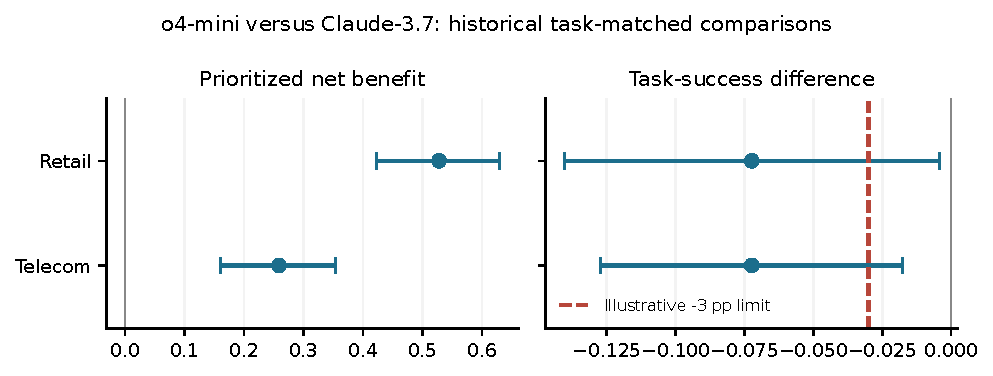
\includegraphics[width=\linewidth]{../results/public_guardrail_reversal.pdf}
\caption{Historical agent comparisons: net benefit and success-rate
difference can favor opposite systems. Intervals are pointwise task
bootstrap summaries, conditional on the archived run configurations;
they do not supply simultaneous or production-population guarantees.}
\label{fig:public}
\end{figure}

The two reversals persist for cost tolerances from 0\% to 20\%. Changing
the priority itself matters: placing tool-call count before cost changes
the telecom o4-mini--Claude-3.7 net benefit from $0.259$ to $-0.126$.
This is a different preference question, not an estimator inconsistency.
SWE-agent Claude-3-Opus versus GPT-4 has net benefit $-0.113$ and success
difference $-0.063$ on the archived runs. These case studies retain
historical model, harness, and price limitations; they do not assert a
ranking of current models.
